\documentclass[margin=0.5mm]{standalone}

\usepackage{pgfplots}
\usepgfplotslibrary{statistics}

\pgfplotsset{
    rshift/.style={
        xshift=-\pgfkeysvalueof{/pgfplots/rshift scale},
        legend image post style={xshift=-\pgfkeysvalueof{/pgfplots/rshift scale}}
        
    },
    lshift/.style={
        xshift=-\pgfkeysvalueof{/pgfplots/lshift scale},
        legend image post style={xshift=\pgfkeysvalueof{/pgfplots/lshift scale}}
      
    },
    rshift scale/.initial=0em,
    lshift scale/.initial=0.4em,
}

%add
%\pgfplotsset{every tick label/.append style={font=\tiny}}

\pgfplotsset{compat=1.7}
\definecolor{BoxCol}{RGB}{47,90,178}
\definecolor{BoxCol1}{RGB}{140,40,40}

\begin{document}
 \thispagestyle{empty}

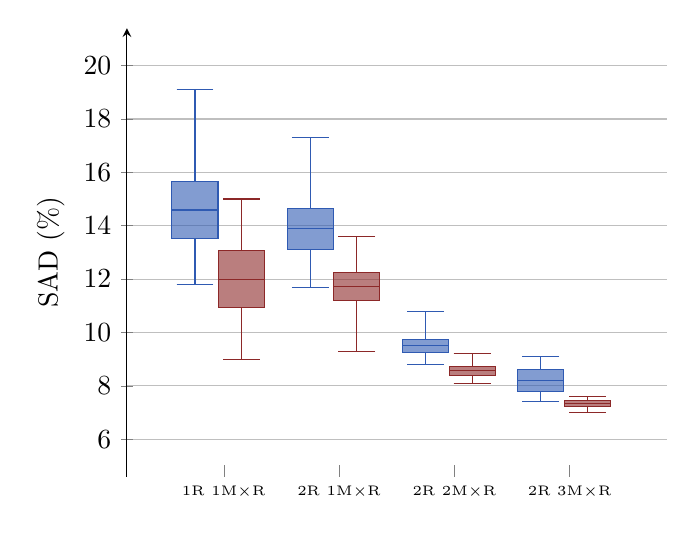
\begin{tikzpicture}

\begin{axis}[
boxplot/draw direction=y,
x axis line style={opacity=0},
%grid = both
axis x line*=bottom,
axis y line=left,
enlarge y limits,
ymajorgrids,
%xtick={1,3,5,7},
xticklabel style = {font=\tiny},
xtick={1.5,3.5,5.5,7.5},
xticklabels={1R 1M$\times$R, 2R 1M$\times$R, 2R 2M$\times$R, 2R 3M$\times$R},
ylabel={SAD (\%)},
ytick={6,8,10,12,14,16,18,20},ymin=6,ymax=20]
]
%BLUE MLP
%RED CNN
    \addplot+[
    rshift,
    boxplot prepared={
      median=14.59,
      upper quartile=14.59+1.06,
      lower quartile=14.59-1.06,
      upper whisker=19.1,
      lower whisker=11.8
    },fill=BoxCol,draw=BoxCol,fill opacity=0.6, solid
    ] coordinates {};
    \addplot+[
       lshift,
    boxplot prepared={
          median=12.0,
      upper quartile=12.0+1.07,
      lower quartile=12.0-1.07,
      upper whisker=15,
      lower whisker=9
    }, fill=BoxCol1,draw=BoxCol1,fill opacity=0.6, solid
    ] coordinates {};
    \addplot+[
        rshift,
    boxplot prepared={
      median=13.88,
      upper quartile=13.88+0.77,
      lower quartile=13.88-0.77,
      upper whisker=17.3,
      lower whisker=11.7
    }, fill=BoxCol,draw=BoxCol,fill opacity=0.6, solid
    ] coordinates {};
        \addplot+[
            lshift,
    boxplot prepared={
      median=11.73,
      upper quartile=11.73+0.52,
      lower quartile=11.73-0.52,
      upper whisker=13.6,
      lower whisker=9.3
    }, fill=BoxCol1,draw=BoxCol1,fill opacity=0.6, solid 
    ] coordinates {};

    \addplot+[
    rshift,
    boxplot prepared={
      median=9.5,
      upper quartile=9.5+0.25,
      lower quartile=9.5-0.25,
      upper whisker=10.8,
      lower whisker=8.8
    },fill=BoxCol,draw=BoxCol,fill opacity=0.6, solid
    ] coordinates {};
    \addplot+[
        lshift,
    boxplot prepared={
      median=8.57,
      upper quartile=8.57+0.17,
      lower quartile=8.57-0.17,
      upper whisker=9.2,
      lower whisker=8.1
    }, fill=BoxCol1,draw=BoxCol1,fill opacity=0.6, solid
    ] coordinates {};
    \addplot+[
        rshift,
    boxplot prepared={
      median=8.2,
      upper quartile=8.2+0.41,
      lower quartile=8.2-0.41,
      upper whisker=9.1,
      lower whisker=7.4
    }, fill=BoxCol,draw=BoxCol,fill opacity=0.6, solid
    ] coordinates {};
    \addplot+[
            lshift,
    boxplot prepared={
      median=7.35,
      upper quartile=7.35+0.11,
      lower quartile=7.35-0.11,
      upper whisker=7.6,
      lower whisker=7
    }, fill=BoxCol1,draw=BoxCol1,fill opacity=0.6, solid
    ] coordinates {};

    \end{axis}
\end{tikzpicture}

%this is for microphone selection simu


\end{document}